% Thishoo IS SIGPROC-SP.TEX - VERSION 3.1
% WORKS WITH V3.2SP OF ACM_PROC_ARTICLE-SP.CLS
% APRIL 2009
%
% It is an example file showing how to use the 'acm_proc_article-sp.cls' V3.2SP
% LaTeX2e document class file for Conference Proceedings submissions.
% ----------------------------------------------------------------------------------------------------------------
% This .tex file (and associated .cls V3.2SP) *DOES NOT* produce:
%       1) The Permission Statement
%       2) The Conference (location) Info information
%       3) The Copyright Line with ACM data
%       4) Page numbering
% ---------------------------------------------------------------------------------------------------------------
% It is an example which *does* use the .bib file (from which the .bbl file
% is produced).
% REMEMBER HOWEVER: After having produced the .bbl file,
% and prior to final submission,
% you need to 'insert'  your .bbl file into your source .tex file so as to provide
% ONE 'self-contained' source file.
%
% Questions regarding SIGS should be sent to
% Adrienne Griscti ---> griscti@acm.org
%
% Questions/suggestions regarding the guidelines, .tex and .cls files, etc. to
% Gerald Murray ---> murray@hq.acm.org
%
% For tracking purposes - this is V3.1SP - APRIL 2009

\documentclass{acm_proc_article-sp}
\usepackage{multirow}
\usepackage{url}
\usepackage{paralist}
\usepackage{statex2}
\usepackage{float}
\begin{document}

\title{Towards an Understanding of Facets and Exemplars of Big Data Applications}
%\subtitle{[Extended Abstract]}
%
% You need the command \numberofauthors to handle the 'placement
% and alignment' of the authors beneath the title.
%
% For aesthetic reasons, we recommend 'three authors at a time'
% i.e. three 'name/affiliation blocks' be placed beneath the title.
%
% NOTE: You are NOT restricted in how many 'rows' of
% ''name/affiliations'' may appear. We just ask that you restrict
% the number of 'columns' to three.
%
% Because of the available 'opening page real-estate'
% we ask you to refrain from putting more than six authors
% (two rows with three columns) beneath the article title.
% More than six makes the first-page appear very cluttered indeed.
%
% Use the \alignauthor commands to handle the names
% and affiliations for an 'aesthetic maximum' of six authors.
% Add names, affiliations, addresses for
% the seventh etc. author(s) as the argument for the
% \additionalauthors command.
% These 'additional authors' will be output/set for you
% without further effort on your part as the last section in
% the body of your article BEFORE References or any Appendices.

\numberofauthors{4} %  in this sample file, there are a *total*
% of EIGHT authors. SIX appear on the 'first-page' (for formatting
% reasons) and the remaining two appear in the \additionalauthors section.
%
\author{
% You can go ahead and credit any number of authors here,
% e.g. one 'row of three' or two rows (consisting of one row of three
% and a second row of one, two or three).
%
% The command \alignauthor (no curly braces needed) should
% precede each author name, affiliation/snail-mail address and
% e-mail address. Additionally, tag each line of
% affiliation/address with \affaddr, and tag the
% e-mail address with \email.Geoffrey C.Fox1, Shantenu Jha2, Judy Qiu1, Andre Luckow2
%(1) School of Informatics and Computing, Indiana University, Bloomington, IN 47408, USA,
%(2) RADICAL, Rutgers University, Piscataway, NJ 08854, USA
%
% 1st. author
\alignauthor
Geoffrey C.Fox\\
       \affaddr{School of Informatics and Computing}\\
       \affaddr{Indiana University, Bloomington}\\
       \affaddr{IN 47408, USA}\\
% 2nd. author
\alignauthor
Shantenu Jha\\
       \affaddr{RADICAL, Rutgers University}\\
       \affaddr{Piscataway}\\
       \affaddr{NJ 08854, USA}\\
% 3rd. author
\alignauthor Judy Qiu\\
       \affaddr{School of Informatics and Computing}\\
       \affaddr{Indiana University, Bloomington}\\
       \affaddr{IN 47408, USA}\\
\and  % use '\and' if you need 'another row' of author names
% 4th. author
\alignauthor Andre Luckow\\
       \affaddr{RADICAL, Rutgers University}\\
       \affaddr{Piscataway}\\
       \affaddr{NJ 08854, USA}\\
% 5th. author
%\alignauthor Sean Fogarty\\
%       \affaddr{NASA Ames Research Center}\\
%       \affaddr{Moffett Field}\\
%       \affaddr{California 94035}\\
%       \email{fogartys@amesres.org}
% 6th. author
%\alignauthor Charles Palmer\\
%       \affaddr{Palmer Research Laboratories}\\
%       \affaddr{8600 Datapoint Drive}\\
%       \affaddr{San Antonio, Texas 78229}\\
%       \email{cpalmer@prl.com}
}

\maketitle
\begin{abstract}
We study many Big Data applications from a variety of research and commercial areas and suggest a set of characteristic features and possible kernel benchmarks that stress those features for data analytics. We draw conclusions for the hardware and software architectures that are suggested by this analysis.
\end{abstract}


\section{Introduction}
With the proliferation of data intensive applications, there is a critical and
timely need to understand these properties and the relationship between
different applications. The aim of our work is to capture the essential and
fundamental Big Data application properties, and then to understand
applications with those properties. There are many different types of Big Data
applications, and we cover them broadly including both research and commercial
cases. However our focus is on Science and Engineering research data-intensive
applications. We compare and contrast some general properties of Big Data
applications with classical HPC simulation applications. Pulling together these
observations, we identify five key system architectures and note different
emphases of commercial and research use cases. However we point out that
combining ideas from HPC and commercial Big Data systems leads to an attractive
powerful Big Data software model. Section~2 describes the sources of
information for our study and their properties. It also describes lessons from
related studies of parallel computing. Section~3 describes the features of Big
Data use cases and the 3 facets into which we group them. We describe some
generic kernels (mini-applications), termed Ogres, in the data analytics area.
In section 4, we present implications for needed hardware and software while
conclusions are in section 5.


\section{Sources of Information}

%\subsection{Data Intensive Use Cases}
In discussing the structure of Big Data applications, let us first discuss the inevitably incomplete input that we used to do our analysis. We have gained of course quite a bit of experience from our research over many years, but 3 explicit sources that we used were a recent use case survey by NIST from Fall 2013~\cite{bb}; a survey of data intensive research applications by Jha et al.~\cite{b28,b26}; and study of members of data analytics libraries including R~\cite{b4}, Mahout~\cite{b1} and MLLib~\cite{b3}. We follow with a summary of first two sources.
The NIST Big Data Public Working Group (NBD-PWG) was launched in June 2013 with a set of working groups covering Big Data Definitions, Taxonomies, Requirements, Security and Privacy Requirements, Reference Architectures White Paper Survey, Reference Architectures, Security and Privacy Reference Architectures and Big Data Technology Roadmap. The Requirements working group gathered 51 use cases from a public call and then analyzed in terms of requirements of a reference architecture~\cite{b21}. Here we will look at them differently to identify common patterns and characteristics, which can be used to guide and evaluate Big Data hardware and software. The 51 use cases are organized into nine broad areas with the number of associated use cases in parentheses: Government Operation (4), Commercial (8), Defense (3), Healthcare and Life Sciences (10), Deep Learning and Social Media (6), The Ecosystem for Research (4), Astronomy and Physics (5); Earth, Environmental and Polar Science (10) and Energy (1). 
Note that the majority of use cases come from research applications but commercial, defense and government operations have some coverage. A template was prepared by the requirements working group, which allowed experts to categorize each use case by 26 features that included those below.
Use case Actors/Stakeholders and their roles and responsibilities; use case goals and description. Specification of current analysis covering compute system, storage, networking and software.  Characteristics of use case Big Data with Data Source (distributed/centralized), Volume (size), Velocity (e.g. real time), Variety (multiple datasets, mashup), Variability (rate of change). The so-called Big Data Science (collection, curation, analysis) with Veracity (Robustness Issues, semantics), Visualization, Data Quality (syntax), Data Types and Data Analytics. These detailed specifications were complemented by broad comments including Big Data Specific Challenges (Gaps), Mobility issues, Security and Privacy Requirements and identification of issues for generalizing this use case.
The complete set of 51 responses with in addition a summary from the working group of applications, current status and futures as well as extracted requirements can be found in~\cite{b21}. They are summarized in the Appendix which also gives 20 other use cases coming from the NBD-PWG which do not have the detailed 26 feature template recorded. These 20 cover enterprise data applications and security and privacy.

% \begin{table}[h]
% \centering
% \caption{ Computational Giants of Massive Data Analysis~\cite{b13}}
% \label{Table5}
% \begin{tabular}{|c|p{5cm}|} \hline
% G1 & Basic Statistics \\ \hline
% G2 & Generalized N-Body Problems \\ \hline
% G3 & Graph-Theoretic Computations \\ \hline 
% G4 & Linear Algebraic Computations \\ \hline
% G5 & Optimizations \\ \hline
% G6 & Integration \\ \hline
% G7 & Alignment Problems 
% \\ \hline
% \end{tabular}
% \end{table}

The impressive NRC report~\cite{b13} is a rich source of information. It has in chapter 2 several examples; most of these are also present in NIST study but NRC does have an interesting discussion of Big Data in Networking and Telecommunication that is omitted from NIST compilation. We will return to the important ``Giants'' in chapter 10 which are related to different facets of our Ogres.
For the case of distributed applications there are at least two existing attempts to survey and analyze applications. In Jha et\,al.~\cite{b26}, the authors examine at a high-level approximately 20 distinct scientific applications that have either been distributed by design or were distributed ``by nature''.  They reduce the number of applications carefully examined to six representative applications. These applications range from the ubiquitous ``$@$home'' class of distributed applications, to Montage - an image reconstruction application which is now emblematic of loosely coupled workflows, to highly-specialized and performance oriented applications such as NEKTAR. 
Building upon~\cite{b26}, Jha et\,al.~\cite{b28} seek to understand distributed, dynamic and data-intensive applications (D3 Science) investigating the programming models and abstractions, the run-time and middleware services, and the computational infrastructure. The survey includes the following applications: NGS Analytics, CMB, Fusion, Industrial Incident Notification and Response, MODIS Data Processing, Distributed Network Intrusion Detection, ATLAS/WLCG, LSST, SOA Astronomy, Sensor Network Application, Climate, Interactive Exploration of Environmental Data, and Power Grids. 

\subsection{Lessons from Parallel Computing}
Before discussing features and patterns of Big Data applications, it
is instructive to consider the better understood parallel computing
situation. Here the application requirements have been captured in
many ways

\begin{compactenum}
\item \textbf{Benchmark Sets.} These vary from full applications~\cite{b9} to
kernels or mini-applications such as the NAS Parallel Benchmark~\cite{b20,b25}
or Parkbench~\cite{b5} with the Top500~\cite{b16} pacing application Linpack
(HPL) particularly well known~\cite{b6}. The new sparse HPCG conjugate gradient
benchmark is notable~\cite{b6}. Note benchmarks can be specified via explicit
code and/or specified by a ``pencil and paper specification'' that can be
optimized in any way for a particular platform. 
\item \textbf{Patterns or Templates.} These can be similar to benchmarks but
with different goals such as providing a generic framework that can be modified
by users with details of their application as in Template book~\cite{b24,b29}.
Alternatively they can be aimed at illustrating different applications as in
original Berkeley Dwarfs~\cite{b8}.
\end{compactenum}


In this paper, our approach is nearest that of the Dwarfs and one motivation
for us calling our mini-applications/kernels the Big Data Ogres. In looking at
this previous work, we note that benchmarks often cover a variety of different
application aspects and are accompanied by principles or folklore that can
guide the writing of parallel code or designing suitable hardware and software.
For example, data locality and cost of data movement, sparseness, Amdahl's law,
communication latency and bisection bandwidth and scaled speedup are associated
with substantial folklore. The famous NAS Parallel Benchmarks (NPB) consists of
MG: Multigrid, CG: Conjugate Gradient, FT: Fast Fourier Transform, IS: Integer
sort, EP: Embarrassingly Parallel, BT: Block Tridiagonal, SP: Scalar
Pentadiagonal, and LU: Lower-Upper symmetric Gauss Seidel, are pretty uniform.
With the exception of EP, which is an application class, the other members are
typical constituents of a low level library for parallel simulations. On the
other hand the Berkeley Dwarfs are Dense Linear Algebra , Sparse Linear
Algebra, Spectral Methods, N-Body Methods, Structured Grids, Unstructured
Grids, MapReduce, Combinational Logic, Graph Traversal, Dynamic Programming,
Backtrack and Branch-and-Bound, Graphical Models and Finite State Machines. The
dwarfs are not exact kernels but describe problem from different points of view
including programming model (MapReduce), numerical method (Grids, Spectral
method), kernel structure (dense or sparse linear algebra), algorithm (dynamic
programming) and application class (N-body) etc. We think that it is inevitable
that both parallel computing and Big Data cannot be characterized with a single
criterion and so we introduce multiple Orges, but with a common set of facets
in several characterization directions. We anticipate that there will be a
correlation between the specific facet values and Ogre type/characterization.


\subsection{Properties of the 51 NIST Use Cases}

\begin{table}[t]
\centering
\caption{What is Parallelism Over for NIST Use Cases}
\label{Table1}
%\begin{tabular}{|c|p{10cm}|} \hline
\begin{tabular}{|p{2.0cm}|p{5.75cm}|} \hline
\textbf{General Class} & \textbf{Examples}\\ \hline
People & Users (but see below) or Subjects of application and often both\\ \hline
Decision makers & Researchers or doctors (users of application)\\ \hline
%\multirow {Items}  & Experimental observations\\ & Contents of online store\\ & Images or Electronic Information nuggets \\ & EMR: Electronic Medical Records (often similar to people parallelism)\\ & Protein or Gene Sequences\\ & Material properties, Manufactured Object specifications, etc., in custom dataset \\ \hline 
Items  & Experimental observations\newline Contents of online store\newline  Images or Electronic Information nuggets \newline EMR: Electronic Medical Records (often similar to people parallelism)\newline Protein or Gene Sequences\newline Material properties, Manufactured Object specifications, etc., in custom dataset \\ \hline 
Modeled entities & Vehicles and people \\ \hline
Sensors & Internet of Things \\ \hline
Events & Detected anomalies in telescope, credit card or atmospheric data \\ \hline
Graph Nodes & RDF databases \\ \hline
Regular Nodes & Simple nodes as in a learning network \\ \hline
Information Units & Tweets, Blogs, Documents, Web Pages, etc. and characters/words in them \\ \hline
Files or data & To be backed up, moved or assigned metadata \\ \hline
Particles/cells/ mesh points & Used in parallel simulations\\
\hline\end{tabular}
\end{table}

Tables~\ref{Table1} to~\ref{Table3} summarize characteristics of the 51 use cases, which we will combine with other input for the Ogres. Note that Big Data and parallel programming are intrinsically linked as any Big Data analysis is inevitably processed in parallel. Parallel computing is almost always implemented by dividing the data between processors (data decomposition); the richness here is illustrated in Table~\ref{Table1} which lists the members of space that is decomposed for different use cases; of course these sources of parallelism are broadly applicable outside the 51 use cases they were extracted from. In Table~\ref{Table2}, we identify 15 use case features that will be used later as components of the Ogre facets. The second column of Table~\ref{Table2} lists our estimate of the number of use cases that illustrate this feature; note these are not exclusive so any one use case will illustrate many features.
It's important to note that machine learning is commonly used but there is an interesting distinction between what are termed Local (LML) and Global machine learning (GML) in Table~\ref{Table2}. In LML, there is parallelism over items of Table~\ref{Table1} and machine learning is applied separately to each item; needed machine learning parallelism is limited and is typified by use of accelerators (GPU). In GML, the machine learning is applied over the full dataset with MapReduce, MPI or equivalent. Typically GML comes from maximum likelihood or $\chisq$ with a sum over the data items - documents, sequences, items to be sold, images etc. and often links (point-pairs). Usually GML is a sum of positive numbers as in least squares and is illustrated by algorithms like PageRank, clustering/community detection, mixture models, topic determination, Multidimensional scaling, and (Deep) Learning Networks. Somewhat quixotically, GML can be termed Exascale Global Optimization or EGO. 

\begin{table}[t]
\centering
\caption{Some Features of NIST Use Cases}
\label{Table2}
\begin{tabular}{|p{1.5cm}|c|p{5.75cm}|} \hline
\textbf{Abbrev. } & \textbf{\#} & \textbf{Description} \\ \hline
PP & 26 & Pleasingly Parallel or Map Only \\ \hline
MR & 18 & Classic MapReduce MR (add MRStat below for full count) \\ \hline
MRStat & 7 & Simple version of MR where key computations are simple reduction as found in statistical averages such as histograms and averages  \\ \hline
MRIter & 23 & Iterative MapReduce or MPI \\ \hline
Graph & 9 & Complex graph data structure needed in analysis \\ \hline
Fusion & 11 & Integrate diverse data to aid discovery/decision making; could involve sophisticated algorithms or could just be a portal \\ \hline
Streaming & 41 &Some data comes in incrementally and is processed this way \\ \hline
Classify & 30 & Classification: divide data into categories \\ \hline
S/Q & 12 & Index, Search and Query \\ \hline
CF & 4 & Collaborative Filtering for recommender engines \\ \hline
LML & 36 & Local Machine Learning (Independent for each parallel entity) \\ \hline
GML & 23 & Global Machine Learning: Deep Learning, Clustering, LDA, PLSI, MDS, Large Scale Optimizations as in Variational Bayes, MCMC, Lifted Belief Propagation, Stochastic Gradient Descent, L-BFGS, Levenberg-Marquardt . Can call EGO or Exascale Global Optimization with scalable parallel algorithm \\ \hline
    & 51 &Workflow: Universal so no label \\ \hline
GIS & 16 & Geotagged data and often displayed in ESRI, Microsoft Virtual Earth, Google Earth, GeoServer etc. \\ \hline
HPC & 5 & Classic large-scale simulation of cosmos, materials, etc. generating (visualization) data \\ \hline
Agent & 2 & Simulations of models of data-defined macroscopic entities represented as agents \\ 
\hline\end{tabular}
\end{table}


The difference between LML and GML is illustrated in Table~\ref{Table3}, which contrasts 9 of the 51 NIST use cases that involve image based data. For example, use case 18 with light source data is largely independent machine learning on each image from the source i.e. LML. In contrast deep learning in use case 26, is constructing a learning network integrating all the images.

%TABLE 3

\begin{table*}
\centering
\caption{9 Image-based NIST Use Cases}
\label{Table3}
\begin{tabular}{|c|p{3cm}|p{7cm}|p{2cm}|} \hline
\textbf{Use Case} & \textbf{Title} & \textbf{Application} & \textbf{Features} \\ \hline
17 & Pathology Imaging/ Digital Pathology & Moving to terabyte size 3D images, Global Classification & PP, LML, MR for search \\ \hline
18 & Light sources & Biology and Materials & PP, LML \\ \hline
26 & Large-scale Deep Learning & Stanford ran 10 million images and 11 billion parameters on a 64 GPU HPC; vision (drive car), speech, and Natural Language Processing & GML \\ \hline
27 & Organizing large-scale, unstructured collections of photos & Fit position and camera direction to assemble 3D photo ensemble & GML \\ \hline
36 & Catalina Real-Time Transient Synoptic Sky Survey (CRTS) & Processing of individual images for events based on classification of image structure (GML) & PP, LML, GML \\ \hline
43 & Radar Data Analysis for CReSIS Remote Sensing of Ice Sheets & Identify glacier beds and snow layers \newline See GML when one addresses full ice sheet & PP, LML moving to GML \\ \hline
44 & UAVSAR Data Processing & Find and display slippage from radar images. Includes Data Product Delivery, and Data Services & PP \\ \hline
45, 46 & Analysis of Simulation visualizations & Find paths, classify orbits, classify patterns that signal earthquakes, instabilities, climate, turbulence & PP,LML,GML \\ \hline
\end{tabular}
\end{table*}



\subsection{Properties of Distributed Use Cases}
%TABLE 4
\begin{table*}
\centering
\caption{Characteristics of 6 Distributed Applications}
\label{Table4}
\begin{tabular}{|p{2cm}|p{2cm}|p{3cm}|p{2cm}|p{3cm}|} \hline
\textbf{Application Example} & \textbf{Execution Unit} & \textbf{Communication} & \textbf{Coordination} & \textbf{Execution Environment} \\ \hline
Montage & Multiple sequential and parallel executable & Files & Dataflow (DAG) & Dynamic process creation, execution \\ \hline
NEKTAR  & Multiple concurrent parallel executables & Stream based & Dataflow & Co-scheduling, data streaming, async. I/O \\ \hline
Replica-Exchange & Multiple seq. and parallel executables & Pub/sub & Dataflow and events & Decoupled coordination and messaging \\ \hline
Climate Prediction (analysis)& Multiple seq. and parallel executables & Files and messages & Dataflow & Dynamics process creation, workflow execution \\ \hline
SCOOP & Multiple Executable & Files and messages & Dataflow & Preemptive scheduling, reservations \\ \hline
Coupled Fusion & Multiple executable & Stream-based & Dataflow & Co-scheduling, data streaming, async I/O
\\ \hline
\end{tabular}
\end{table*} 

In the process of reduction and classification, the authors of~\cite{b28,b26}
analyze the structure of applications and find commonalities; they introduce
the term ``vectors'' to capture four essentially orthogonal but critical
properties that determine both the development and the execution of the
application. These vectors are: execution unit, communication, coordination and
an execution environment. The first three are internal properties of a
distributed application, whereas the latter is essentially an external
property. Based upon recurring values of vectors the authors propose a set of
common patterns that help elucidate the structure of the distributed
applications. It is worth noting, that vectors and patterns for distributed
applications do not provide insight into performance aspects of the
applications. In~\cite{b28}, the authors propose a framework for describing
applications, distributed and dynamic data and infrastructure. Figure 1 shows
the data lifecycle model used for the analysis capturing both applications
using sensor and computationally generated data.


%DIAGRAM Figure Application Stages
\begin{figure}
\centering
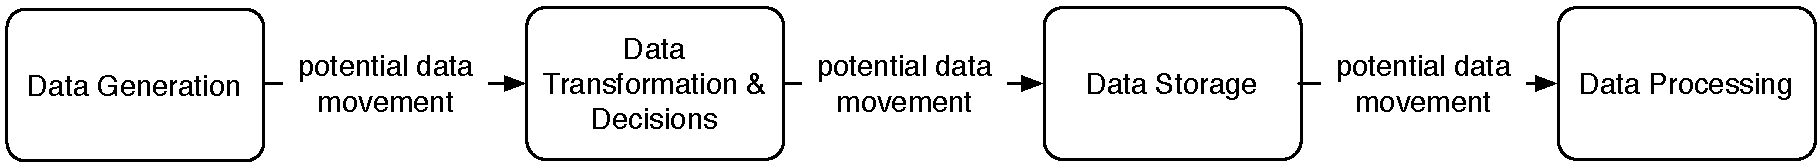
\includegraphics[width=0.5\textwidth]{fig1.pdf}
\caption{Figure Application Stages}
\label{figure1}
\end{figure}

The authors call out the Big Data aspects, the dynamic aspects and the
distributed aspects of a large set of applications, and introduce quantitative
estimates for various performance related properties. The Table~\ref{Table4}
below (from~\cite{b26}) shows the specific values of the ``DPA vectors'' for
the set of six distinct applications investigated. It is interesting to note
that the categorization did not lead to well-defined and non-overlapping
classification of application, as the complexity of considering the end-to-end
aspects and the diverse ways in which applications are utilized, resulted in
classes that had overlapping characteristics.



\section{The Big Data Ogres and their Three Facets}

%TABLE 5
% \begin{table*}
% \centering
% \caption{ Computational Giants of Massive Data Analysis~\cite{b13}}
% \label{Table5}
% \begin{tabular}{|c|p{5cm}|} \hline
% G1 & Basic Statistics \\ \hline
% G2 & Generalized N-Body Problems \\ \hline
% G3 & Graph-Theoretic Computations \\ \hline 
% G4 & Linear Algebraic Computations \\ \hline
% G5 & Optimizations \\ \hline
% G6 & Integration \\ \hline
% G7 & Alignment Problems 
% \\ \hline
% \end{tabular}
% \end{table*}

Synthesizing lessons learned from HPC, distributed applications and the NIST use case, given above we argue that there is a need to construct classes of mini-applications that facilitate the understanding and characterization of the Big Data properties of these applications. We further introduce 3 facets or classification dimensions or features to categorize Big Data applications. These are Problem architecture, Computational features and Data Source or Style. There are of course other ways of looking at the Ogres and our work should be treated as an initial suggestion for further discussion. These facets build on earlier discussion - especially Table 2.

\begin{table}[h]
\centering
\caption{ Computational Giants of Massive Data Analysis~\cite{b13}}
\label{Table5}
\begin{tabular}{|c|p{5cm}|} \hline
G1 & Basic Statistics \\ \hline
G2 & Generalized N-Body Problems \\ \hline
G3 & Graph-Theoretic Computations \\ \hline 
G4 & Linear Algebraic Computations \\ \hline
G5 & Optimizations \\ \hline
G6 & Integration \\ \hline
G7 & Alignment Problems 
\\ \hline
\end{tabular}
\end{table}

Note that a given application can be made up of components with different
characteristics in Ogre Facet classification. We will reference the 7
computational giants G1-G7 from the NRC report~\cite{b13} recorded in
Table~\ref{Table5}. These are important big data patterns but the Ogres go into
more detail. The final subsection discusses a selection of kernel Ogres
focusing on analytics. We intend to follow up with other Ogres ``mini-apps'' or
``kernels'' covering areas like data intensive workflows.


\subsection{Problem Architecture Facet of Ogres}

Table~\ref{Table6} summarized the identified problem architectures of the Ogres.

%TABLE 6
\begin{table}[t]
\centering
\caption{Problem Architecture Facet of Ogres (Meta or Macro Pattern)}
\label{Table6}
\begin{tabular}{|p{1.5cm}|p{5.75cm}|} \hline
Pleasingly Parallel & as in BLAST, Protein docking, some (bio-)imagery  including Local Analytics or Local Machine Learning with pleasingly parallel filtering, as in light source data, radar images \\ \hline 
Classic MapReduce & Search, Index and Query and Classification algorithms like collaborative filtering (G1 for MRStat in Table~\ref{Table2}, G7) \\ \hline
GML & Global Analytics or Global Machine Learning requiring iterative runtime (G5, G6) \\ \hline
Graph & Problem set up as a graph as opposed to vector, grid (G3) \\ \hline
SPMD & SPMD (Single Program Multiple Data) \\ \hline
BSP & Bulk Synchronous Processing: well-defined compute-communication phases \\ \hline
Fusion or Workflow & Knowledge discovery often involves fusion of multiple methods. All applications often involve orchestration (workflow) of multiple components \\ \hline
Agents & As used in epidemiology, discrete event simulations etc. Swarm approaches
\\ \hline
\end{tabular}
\end{table}


\subsection{Computational features Facet of Ogres}
%TABLE 7
\begin{table}[H]
\centering
\caption{ Computational Features Facet of Ogres}
\label{Table7}
\begin{tabular}{|p{8cm}|} \hline
Flops per byte: important for performance \\ \hline
Communication Interconnect requirements; \\ \hline
Is application (graph) constant or dynamic? \\ \hline
Most applications consist of a set of interconnected entities; is this regular as a set of pixels or is it a complicated irregular graph? \\ \hline
Is communication BSP or Asynchronous? In latter case shared memory may be attractive;\\ \hline
Are algorithms Iterative or not?\\ \hline
Are algorithms governed by dataflow?\\ \hline
Data Abstraction: key-value, pixel, graph, vector, HDF5 etc.\\ \hline
Are data points in metric or non-metric spaces (G2)? \\ \hline
Is algorithm O(N2) or O(N) (up to logs) for N points per iteration (G2)\\ \hline
Core libraries needed: matrix-matrix/vector algebra, conjugate gradient, reduction, broadcast. (G4)
\\ \hline
\end{tabular}
\end{table}


This facet contains application characteristics that are familiar from the
simulation domain. Distinctive are the important data abstraction layer that we
would recommend highlighting in the software architecture rather than burying
as now in particular packages like Hadoop (key-value) and Giraph (graph).
Simulations are often setup in well-defined physical spaces but data is often
more abstract and the algorithms are typically quite different for metric and
non-metric spaces. In contrast to the problem architecture facet, the
computational features facet have a direct handle/relevance to performance.
Note non-metric space algorithms are often O(N2). As discussed in the NRC
report, there is a lot of opportunity to incorporate sophisticated new
algorithms to reduce O(N2) to O(N and logs). This is commonly used in search
and sort algorithms but not yet in computation in spite of promising initial
work~\cite{b13,b23,b19}.


\subsection{Data Source and Data Style Facet of Ogres}

The facet of Table~\ref{Table8} covers the acquisition, storage, management and
access to the data. The mantra of bringing computing to the data is an
important principle especially for the Internet of Things when it is often not
practical as backend (clouds) needed to provide adequate computing. It is
interesting that the HPC approach of large shared file systems using
technologies like Lustre is rather different from commercial systems that use
databases or increasingly HDFS. Figure 1 stresses that an important source of
data is the output of other programs as data is streamed through a workflow and
requires in-motion analytics, e.\,g.\ the update of an analytical model, and
the delivery of a realtime response. The lambda
architecture~\cite{marz2013principles} integrates stream processing and batch
processing backend in a unified framework: while the batch layer (e.\,g.\ based
on HDFS) handles processing requirement on the entire data set, the speed layer
provides the ability to analyze in-coming data in-motion.

%TABLE 8
\begin{table}[H]
\centering
\caption{Data Source and Style Facet of Ogres}
\label{Table8}
\begin{tabular}{|p{8cm}|} \hline
SQL or NoSQL: NoSQL includes Document, Column, Key-value, Graph, Triple store \\ \hline
Other Enterprise data systems: 10 examples from NIST~\cite{bb} integrate SQL/NoSQL \\ \hline
Set of Files: as managed in iRODS and extremely common in scientific research \\ \hline
File, Object, Block and Data-parallel (HDFS) raw storage: Separated from computing? \\ \hline
Internet of Things: 24 to 50 billion devices on the Internet by 2020~\cite{b22,b11,b12} \\ \hline
Streaming: Incremental update and analysis of datasets with new algorithms to achieve real-time response (G7) \\ \hline
HPC simulations generate major (visualization) output that often needs to mined \\ \hline
GIS (Geographical Information Systems) provide attractive access to geospatial data \\ \hline
Before data gets to compute system, there is often an initial data gathering phase which is characterized by a block size and timing. Block size varies from month (Remote Sensing, Seismic) today (genomic) to seconds or lower (Real time control, streaming)\\ \hline
There are storage/compute system styles: Shared, Dedicated, Permanent, Transient \\ \hline
Other characteristics are needed for permanent auxiliary/comparison datasets and these could be interdisciplinary, implying nontrivial data movement/replication
\\ \hline
\end{tabular}
\end{table}



\subsection{Analytics Algorithm/Kernel Ogres}

The final Ogre Table~\ref{Table9} records particular data analysis algorithms
that play the same role as say the members of the NAS parallel benchmarks.
These are deliberately kernels and further work is needed to specify more
precisely. For example, there are many very different outlier and clustering
algorithms corresponding to different scenarios (such as metric or non-metric
spaces) and goals (such as tradeoff between performance and quality). We are
developing with colleagues, benchmarks in the areas identified in
Table~\ref{Table9}. One should also introduce Ogres corresponding to full
applications and workflows. These are important but not discussed here. We
believe that the set of facets that will be needed to understand these other
mini-apps will be common across Ogres.

%TABLE 9
\begin{table}[H]
\centering
\caption{Analytics Ogres (microPatterns)}
\label{Table9}
\begin{tabular}{|p{8cm}|} \hline

\textbf{Pleasingly Parallel (Map Only) or Local Machine Learning: ~any algorithm} \\ \hline 
\textbf{Map-Reduce} \\ \hline
Search, Query, Index: Dominant commercial use and important in Science with less users \\ \hline
Recommender Systems including Collaborative filtering: Major commercial use, Little use in Science \\ \hline
Summarizing statistics (MRStat) as in LHC Data analysis (histograms) (G1) \\ \hline
Linear Classifiers: Bayes, Random Forests \\ \hline
\textbf{Alignment and Streaming (G7)} \\ \hline
Genomic Alignment, Incremental Classifiers \\ \hline
\textbf{Global Analytics - Nonlinear Solvers (Structure depends on Objective Function) (G5, G6)} \\ \hline
Stochastic Gradient Descent SGD \\ \hline
(L-)BFGS approximation to Newton's Method \\ \hline
Levenberg-Marquardt solver \\ \hline
\textbf{Global Analytics - Map-Collective (See Mahout, MLlib) (G2, G4, G6)} \\ \hline
Outlier Detection \\ \hline
Clustering (many methods) related to community identification in networks \\ \hline
Mixture Models, LDA (Latent Dirichlet Allocation), PLSI (Probabilistic Latent Semantic Indexing)\\ \hline
SVM and Logistic Regression\\ \hline
PageRank (find leading eigenvector of sparse matrix)\\ \hline
SVD (Singular Value Decomposition)\\ \hline
MDS (Multidimensional Scaling)\\ \hline
Learning Neural Networks (Deep Learning)\\ \hline
Hidden Markov Models\\ \hline
\textbf{Global Analytics - Map-Communication (targets for Giraph) (G3)}\\ \hline
Graph Structure (Communities, subgraphs/motifs, diameter, maximal cliques, connected components)\\ \hline
Network Dynamics - Graph simulation Algorithms (epidemiology)\\ \hline
Global Analytics - Asynchronous Shared Memory (may be distributed algorithms)\\ \hline
Graph Structure (Betweenness centrality, shortest path) (G3)\\ \hline
Linear/Quadratic Programming, Combinatorial Optimization, Branch and Bound (G5)
\\ \hline
\end{tabular}
\end{table}




\section{Hardware and Software Architecture Issues}
\subsection{Five Important Architectures}

%TABLE 10
\begin{table}[h]
\centering
\caption{Distinctive Software/Hardware Architectures for Data Analytics}
\label{Table10}
\begin{tabular}{|p{2.55cm}|p{5.45cm}|} \hline
1. Pleasingly Parallel (Map Only) & Includes local machine learning (LML) as in parallel decomposition over items and apply data processing to each item. Hadoop could be used but also other High Throughput Computing or Many task tools \\ \hline
2. Classic Map\-Reduce & Includes MRStat, search applications and those using collaborative filtering and motif finding implemented using classic MapReduce (Hadoop)\\ \hline
3. Iterative Map-Collective & Iterative MapReduce using Collective Communication as needed in clustering - Hadoop with Harp, Spark etc. \\ \hline
4. Iterative Map\-Communi\-cation & Iterative MapReduce such as Giraph with point-to-point communication and includes most graph algorithms such as maximum clique,  connected component, finding diameter, community detection). Vary in difficulty of finding partitioning (classic parallel load balancing)\\ \hline
5. Shared (Lar\-ge) Memory & Thread-based (event driven) graph algorithms such as shortest path and Betweenness centrality. Large memory applications
 
\\ \hline
\end{tabular}
\end{table}

In Table~\ref{Table10}, we present 5 distinct problem architectures
that map into 5 distinct system architectures which seem to cover the
Ogres and their facets discussed in previous section. 10.5 is the
shared memory architecture needed for some graph algorithms that
perform better here and also for some large memory applications. The
central architectures are 10.1 to 10.4 which correspond exactly to the
four forms of MapReduce that we have presented previously~\cite{b18}
but are summarized in figure 2. Note this only describes some core
features of the facets in Tables~\ref{Table6} and~\ref{Table7}. There
are many other issues that need to be addressed including support of
workflow and the data systems captured in the facets of
Table~\ref{Table8}. In particular the architecture for the rapidly
evolving field of streaming (distributed) data needs more work.


%Figure 2: The Four forms of MapReduce that correspond to the four architectures of Table 10.1-10.4
\begin{figure}
\centering
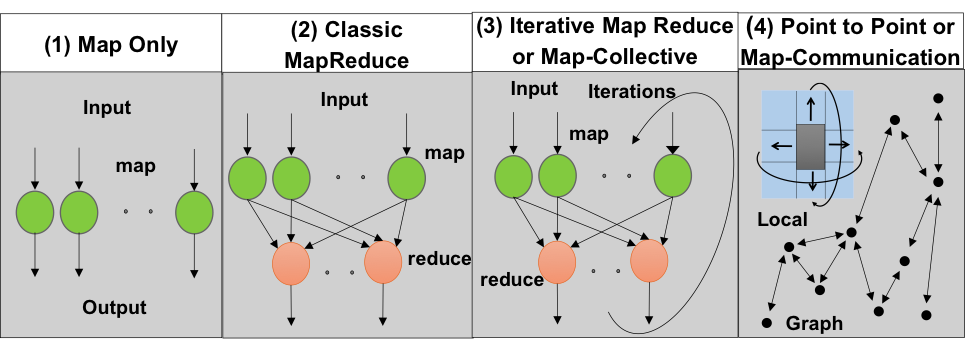
\includegraphics[width=0.5\textwidth]{mapreduce-four.png}
\caption{The Four forms of MapReduce that correspond to the four architectures of Table 10.1-10.4}
\end{figure}


Note that we separate Map-Collective~\cite{b24,b25} and Map-(Point to Point)
Communication following the Apache projects Hadoop, Spark and Giraph that focus
on these cases. These programming models or run times differ in communication
style, application abstraction (key-value versus graph) and possible
scheduling/load-balancing. HPC with MPI suggests that one could integrate 10.3
and 10.4 into a single environment and this approach is illustrated by the Harp
plug-in to Hadoop which supports both models.


\subsection{Comparison between Data Intensive and Simulation Problems}

We can use the Ogre facet analysis and the data analytics architectures to
compare data intensive and simulation applications. There are some clear
similarities with looking back at Table~\ref{Table6}, ``Pleasingly parallel''
(10.1), BSP and SPMD common in both arenas. However, the Classic MapReduce
architecture (10.2) is a major big data paradigm, but has much less common in
simulations with one example between the execution of multiple simulations (as
in Quantum Monte Carlo) followed by a reduce operation to collect the results
of different simulations. The Iterative Map-Collective architecture (10.3) is
common in much Big Data analytics as in clustering where there is no local
graph structure and the parallel algorithms involve large scale collectives but
no point to point communication. The same structure is seen in N-body (long
range force) or other ``all-pairs'' simulations without the locality typical
from discretizing differential operators. Many simulation problems have the
Map-Communication (10.4) architecture with many smallish point-to-point
messages coming from local interactions between points defining system to be
simulated. The importance of sparse data structures and algorithms is well
understood in simulations and is seen in some Big Data problems such as
PageRank, which calculates the leading eigenvector of the sparse matrix formed
by internet site links. Other Big Data sparse data structures are seen in
user-item ratings and bags of words problem. Most items are rated by few users
and many documents contain a small fraction of the word vocabulary. However
important data analytics involve full matrix algorithms and for example recent
papers~\cite{b31,b32} on a new Multi-Dimensional Scaling method use conjugate
gradient solvers with full matrices as opposed to the new sparse conjugate
gradient benchmark HPCG being developed for supercomputer (Top500) evaluations
~\cite{b17}. Note that there are similarities between some Big Data graph
problems and particle simulations with an unusual potential defined by the
graph node connectivity. Both use the Map-Communication architecture and the
links in a Big Data graph are equivalent to strength of force between the graph
nodes considered as particles. In this analogy, many Big Data problems are
``long range force'' corresponding to a graph where all nodes are linked to
each other. As in simulation case, these O(N2) problems are typically very
compute intense but straightforward to parallelize efficiently. It is
interesting to consider the analogue of the ``fast multipole'' methods for the
fully connected Big Data problems which can dramatically improve the
performance to O(N) or O(N\,log\,N) as discussed in Sec. 3.3. Finally note the
network connections used in deep learning are sparse but in recent image
interpretation studies~\cite{b7}, the network weights are block sparse
(corresponding to links to pixel blocks) and can be formulated as full matrix
operations with GPUs and MPI running efficiently with these blocks. The final
architecture 10.5 (Shared Memory) is important in some applications but not
heavily used in either simulations or Big Data although large memory systems
are used extensively in gene assembly applications. The above discussion
focuses on a qualitative comparison of Big Data applications with traditional
simulation (HPC) applications viz., comparing the structure. As can be seen
there are similarities as well as points of distinction. It is likely however,
that there will be significant differences in the ``computational
feature'' facet of the two application classes, viz., the distribution of the
values of different ratios (e.g., ratio of computing to I/O, ratio of memory to
I/O etc.) characterizing the computational feature will be different. We will
investigate both quantitative and qualitative differences in future work.


\subsection{A Big Data Software Environment}

%TABLE 11
% \begin{table*}
% \centering
% \caption{}
% \label{Table11}
% \begin{tabular}{|p{12cm}|} \hline
% Message Protocols: Thrift, Protobuf
% \\ \hline
% \end{tabular}
% \end{table*}

% \begin{figure}
% \centering
% \includegraphics[width=0.5\textwidth]{table11.png}
% \caption{Kaleidoscope of (Apache) Big Data Stack (ABDS) and HPC Technologies}
% \label{figure1}
% \end{figure}


\begin{table}[H]
\caption{Big Data Software Environment: ABDS\label{Table11}}
\begin{tabular}{|p{2cm}|p{6cm}|}
\hline
\textbf{Cross-Cutting Functionalities}
&\textbf{Workflow-Orchestration:} Oozie, ODE, Airavata, OODT (Tools), Pegasus, Kepler, Swift, Taverna, Trident, ActiveBPEL, BioKepler, Galaxy, IPython\\ \cline{2-2} 

&\textbf{Application and Analytics:} Mahout, MLlib , MLbase, CompLearn, R, Bioconductor, ImageJ, Scalapack, PetSc\\ \hline


\multirow{2}{2cm}{\textbf{Message Protocols:} Thrift, Protobuf}
&High level Programming: Hive, HCatalog, Pig, Shark, MRQL, Impala, Sawzall\\ \cline{2-2} 

&\textbf{Basic Programming model and runtime, SPMD, Streaming, MapReduce, MPI:} Hadoop, Spark, Twister, Stratosphere, Tez, Hama, Storm, S4, Samza, Giraph, Pregel, Pegasus\\ \hline

\multirow{2}{2cm}{\textbf{Distributed Coordination:} Zookeeper, JGroups}
&\textbf{Interprocess communication, collectives, point-to-point, publish-subscribe:} Hadoop, Spark, Harp, MPI, Netty, ZeroMQ, ActiveMQ, QPid, Kafka, Kestrel\\ \cline{2-2} 

&\textbf{In-memory databases/caches:} GORA (general object from NoSQL), Memcached, Redis (key value), Hazelcast, Ehcache\\ \hline


\multirow{2}{2cm}{\textbf{Security \& Privacy:} InCommon, OpenStack Keystone, LDAP}
&\textbf{Object-relational mapping: }Hibernate, OpenJPA and JDBC Standard\\ \cline{2-2} 
&\textbf{Extraction Tools:} UIMA, Tika\\ \cline{2-2} 

&\textbf{SQL:} Oracle, MySQL, Phoenix, SciDB\\ \cline{2-2} 
&\textbf{NoSQL:} HBase, Accumulo, Cassandra, Solandra, MongoDB, CouchDB, Lucene, Solr, Berkeley DB, Azure Table, Dynamo, Riak, Voldemort. Neo4J, Yarcdata, Jena, Sesame, AllegroGraph, RYA\\ \hline
\multirow{2}{2cm}{\textbf{Monitoring:} Ambari, Ganglia, Nagios, Inca}
&\textbf{File management:} iRODS\\ \cline{2-2} 
&\textbf{Data Transport:} BitTorrent, HTTP, FTP, SSH, Globus Online (GridFTP)\\ \cline{2-2} 
&\textbf{Cluster Resource Management:} Mesos, Yarn, Helix, Llama, Condor, SGE, OpenPBS, Moab, Slurm, Torque\\ \cline{2-2} 
&\textbf{File systems:} Swift, Cinder, Ceph, FUSE, Gluster, Lustre, GPFS, GFFS\\ \cline{2-2} 
&\textbf{Interoperability:} Whirr, JClouds, OCCI, CDMI\\ \cline{2-2} 
&\textbf{DevOps:} Docker, Puppet, Chef, Ansible, Boto, Libcloud, Cobbler, CloudMesh\\ \cline{2-2} 
&\textbf{IaaS Management from HPC to hypervisors:} OpenStack, OpenNebula, Eucalyptus, CloudStack, vCloud, Amazon, Azure, Google\\ \hline
\end{tabular}

\end{table}


We have described elsewhere~\cite{b30,b14,b27} how we propose to implement Big
Data applications exploiting the HPBDS architecture sketched in
Table~\ref{Table11}~\cite{b2}. This combines the best practice commercial Big
Data software with an emphasis on Apache projects with HPC subsystems.
Table~\ref{Table11} illustrates by green shading those layers where HPC adds
significant value to the Apache stack ABDS. Note that high performance
communication is known to be critical for simulations but it is also essential
for many science big data applications. Commercial applications have large
``search'' (10.2) components corresponding to the huge number of users
accessing commercial Big Data systems. In science, this step is necessary -
especially for good data management - but is a much lower fraction of system
use as the number of scientists accessing data is much lower than number of
users of commercial Big Data.

\section{Discussion and Conclusion}

This is only an initial discussion about our objectives, scope and
methodology, and is by no means a complete or comprehensive body of
work. It is motivated by the fact that there are several existing
efforts at describing and highlighting Big Data applications, yet many
are domain or usage specific. We move beyond any specific set of
applications, and focus on Big Data applications and analytics kernels
Ogres that are generally considered to be of relevance/importance to
science and engineering using a context that includes a limited set of
commercial problems. Using this broad range of Big Data applications
as our working set, this paper is an attempt at distilling the Big
Data properties (facets) and organizing the plethora of disparate Big
Data applications using these properties. Although we validate using
analytics kernels, this classification / organization will in turn
shed light on and help provide better understanding of both the
structure of S\&E Big Data applications, as well as determinants of
their performance. In Section 4, we show how a deeper appreciation of
the Ogre facets will help design and implement better hardware and
software systems.

%%%%APPENDIX 
%%%%%REFERENCES


%To set a wider table, which takes up the whole width of
%the page's live area, use the environment
%\textbf{table*} to enclose the table's contents and
%the table caption.  As with a single-column table, this wide
%table will ``float'' to a location deemed more desirable.
%Immediately following this sentence is the point at which
%Table 2 is included in the input file; again, it is
%instructive to compare the placement of the
%table here with the table in the printed dvi
%output of this document.





% The following two commands are all you need in the
% initial runs of your .tex file to
% produce the bibliography for the citations in your paper.
%\bibliographystyle{abbrv}
\bibliographystyle{IEEEtran}
\bibliography{sigproc}  % sigproc.bib is the name of the Bibliography in this case
% You must have a proper ''.bib'' file
%  and remember to run:
% latex bibtex latex latex
% to resolve all references
%
% ACM needs 'a single self-contained file'!
%
%APPENDICES are optional
%\balancecolumns
%\input{appendix}

%\appendix
%Appendix A




  %OR SECTION??
%Generated by bibtex from your ~.bib file.  Run latex,
%then bibtex, then latex twice (to resolve references)
%to create the ~.bbl file.  Insert that ~.bbl file into
%the .tex source file and comment out
%the command \texttt{{\char'134}thebibliography}.
% This next section command marks the start of
% Appendix B, and does not continue the present hierarchy
%\section{More Help for the Hardy}
%The acm\_proc\_article-sp document class file itself is chock-full of succinct
%and helpful comments.  If you consider yourself a moderately
%experienced to expert user of \LaTeX, you may find reading
%it useful but please remember not to change it.
%\balancecolumns
% That's all folks!
\end{document}
